\textbf{Beispiel 3}\\ \\
a)\\ \\
Die Wärmeleitgleichungen für das Kabel und die Isolation können mithilfe der Wärmeleitgleichung für Zylinderkoordinaten aus der Formelsammlung aufgestellt werden und daher lauten diese
\begin{align*}
	\rho_l c_l \frac{\partial T_l(r,t)}{\partial t} &= \lambda_l \left(\frac{1}{r}\frac{\partial }{\partial r}\left( r\frac{\partial T_l(r,t)}{\partial r}\right) + \frac{1}{r^2}\frac{\partial^2T_l(r,t)}{\partial \varphi^2} + \frac{\partial^2 T_l(r,t)}{\partial z^2}\right) + g \\
	\rho_i c_i \frac{\partial T_i(r,t)}{\partial t} &= \lambda_i \left(\frac{1}{r}\frac{\partial }{\partial r}\left( r\frac{\partial T_i(r,t)}{\partial r}\right) + \frac{1}{r^2}\frac{\partial^2T_i(r,t)}{\partial \varphi^2} + \frac{\partial^2 T_i(r,t)}{\partial z^2}\right)
\end{align*}
Da es sich um ein unendlich langes Kabel handelt, kann die Abhängigkeit der z-Koordinate vernachlässigt werden. Außerdem kann aufgrund der Kabelsymmetrie die Abhängigkeit von $\varphi$ entfallen. \\
An der Stelle $r = 0$ muss
\[
	\frac{\partial T_l}{\partial r}\biggl|_{r=0} = 0
\]
Die Lösung der Wärmeleitgleichung muss 2-mal stetig differnzierbar sein, daher gilt an der Kontaktstelle $r_i = r_l$
\[
	T_l(r,t) = T_i(r,t)
\]
Mittels Konvektion tauscht das Kabel samt Isolation Wärme mit der Umgebung aus und somit muss an der Stelle $r = r_i$
\[
	-\lambda_i\frac{\partial T_i(r,t)}{\partial r}\biggl|_{r = r_i} = -\dot{q}^a(t)
\]
Die Gleichung wurde mithilfe des Wärmeleitgesetzes aus der Formelsammlung aufgestellt. \\ \\
b)\\ \\
Im stationären Fall verschwindet die zeitlichen Ableitungen, daher erhalten wir die Wärmeleitgleichungen
\begin{align*}
	0 &= \lambda_i\left( \frac{1}{r}\frac{\partial }{\partial r}\left( r\frac{\partial T_l(r,t)}{\partial r}\right)\right) + g \\
	0 &= \frac{\partial }{\partial r}\left( r\frac{\partial T_i(r,t)}{\partial r}\right)
\end{align*}
\newpage
\noindent
Nun folgt die Überprüfung ob die beiden bekannten Temperaturprofile die stationären Gleichungen erfüllen.\\
$T_l(r)$:
\begin{align*}
	0 &= \lambda_i\left( \frac{1}{r}\frac{\partial }{\partial r}\left( r\frac{\partial T_l(r,t)}{\partial r}\right)\right) + g \\
	0 &= \lambda_i\left( \frac{1}{r}\frac{\partial }{\partial r}\left(\frac{-2gr^2}{4\lambda_l}\right)\right) + g \\
	0 &= \cancel{\lambda_i}\left( \frac{1}{\cancel{r}}\frac{-g\cancel{r}}{\cancel{\lambda_l}}\right) + g\\
	0 &= -g + g = 0
\end{align*}
$T_i(r)$:
\begin{align*}
	0 &= \frac{\partial }{\partial r}\left( \cancel{r} (T_1 - T_2)\frac{\cancel{r_i}}{\cancel{r}\ln(r_l/r_i)}\frac{1}{\cancel{r_i}}\right) \\
	0 &= 0
\end{align*}
Somit ist bewiesen, dass die beiden gegebenen Temperaturprofile die stationären Wärmeleitgleichungen erfüllen. \\ \\
c)\\ \\
Der Temperaturverlauf sieht wie folgt aus
\begin{figure}[h]
	\centering
	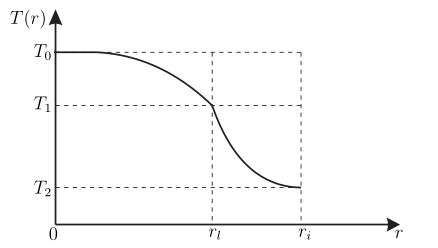
\includegraphics[width=10cm]{tikz/13_05_2016_3c}
\end{figure}
\newline
Unter Berücksichtigung aller Randbedingungen folgt
\[
	T_0 = T_1 + \frac{gr_l^2}{4\lambda_l}
\]
d)\\ \\
Die volumetrische Wärmequelle lautet
\begin{align*}
	g &=  w_l\left(\frac{I}{r_l^2\pi}\right)^2
\end{align*}
Die eingebrachte Energie lautet
\[
	\dot{W} = gr_l^2\pi L = \frac{w_l L}{r_l^2\pi}I^2
\]
e)\\ \\
Die beiden Gesetzmäßigkeiten sind das Reziprozitätsgesetz
\[
	A_iF_{ij} = A_jF_{ji}
\]
und der Summationsregel
\[
	1 = \sum_{j=1}^{N} F_{ij} \qquad \forall \in \{ 1, ... , N\}
\]
Bei konvexen Körpern ist der Sichtfaktor $F_{ii}$ immer gleich 0. \\ \\
f)\\ \\
Die gesuchte Wärmestromdichte wird mithilfe der Nettowärmestromdichte
\[
	\dot{\textbf{q}}_s = (\textbf{E} - \textbf{F})(\textbf{E} - (\textbf{E} - \text{diag}\{\varepsilon\})\textbf{F})^{-1}\text{diag}\{\varepsilon\}\sigma\textbf{T}^4
\]
mit den Vektoren $\dot{\textbf{q}_s} = \left[ \dot{q}_s^a , \dot{q}_s^w\right]^T , \textbf{T} = \left[T_2,T_W\right]^T$ und $\varepsilon = \left[\varepsilon_i , \varepsilon_w\right]^T$ und der Einheitsmatrix
\[
	\textbf{E} = \begin{bmatrix}
		1 & 0 \\
		0 & 1
	\end{bmatrix}
\]
Bestimmung der Sichtfaktoren:
\begin{align*}
	F_{ii} &= 0 \\
	F_{iw} &= 1 \\
	r_i\pi &= (a_w + b_w)F_{wi} \\
	F_{wi} &= \frac{r_i\pi}{a_w + b_w} \\
	F_{ww} &= 1 - \frac{r_i\pi}{a_w + b_w}
\end{align*}
Damit lautet die Sichtfaktormatrix
\[
	\textbf{F} = \begin{bmatrix}
		0 & 1 \\
		\frac{r_i\pi}{a_w + b_w} & 1 - \frac{r_i\pi}{a_w + b_w}
	\end{bmatrix}
\]
g)\\ \\
Die konvektive Wärmestromdichte $\dot{q}_k^a$ lautet
\begin{align*}
	\dot{q}_k^a &= - \alpha(T_2 - T_\infty) \\
				&= \alpha (T_\infty - T_2)
\end{align*}
Somit folgt für den gesamten Wärmestrom $\dot{Q}^a$ an der Stelle $r = r_i$
\[
	\dot{Q}^a = 2r_i\pi L (\dot{q}_k^a +\dot{q}_s^a)
\]